\documentclass[10pt,twocolumn,letterpaper]{article}

\usepackage{cvpr}
\usepackage{times}
\usepackage{epsfig}
\usepackage{graphicx}
\usepackage{amsmath}
\usepackage{amssymb}
\usepackage{booktabs}
\usepackage{float}


% Include other packages here, before hyperref.

% If you comment hyperref and then uncomment it, you should delete
% egpaper.aux before re-running latex.  (Or just hit 'q' on the first latex
% run, let it finish, and you should be clear).
\usepackage[breaklinks=true,bookmarks=false]{hyperref}

\cvprfinalcopy % *** Uncomment this line for the final submission

\def\cvprPaperID{0429} % *** Enter the CVPR Paper ID here
\def\httilde{\mbox{\tt\raisebox{-.5ex}{\symbol{126}}}}

% Pages are numbered in submission mode, and unnumbered in camera-ready
%\ifcvprfinal\pagestyle{empty}\fi
\setcounter{page}{1}
\begin{document}

%%%%%%%%% TITLE
\title{Stock Market Prediction Using LSTM}

\author{Edison Huang\\
Virginia Tech\\
Blacksburg, VA\\
{\tt\small edisonrhuang@vt.edu}
}

\maketitle
%\thispagestyle{empty}

%%%%%%%%% ABSTRACT
\begin{abstract}
   Given the inherent complexity and volatility of financial markets, it is
   difficult to predict stock prices in financial analysis. In this paper, we
   will use Long Short-Term Memory (LSTM) neural networks – a type
   of recurrent neural network (RNN) – for predicting stock prices 
   \cite{parmar2018}. Apple Inc. (AAPL) stock price is the main focus of 
   this research where historical data were used to train and evaluate 
   LSTM model. The report also provides detailed information about 
   data preprocessing steps, model architecture, hyperparameter 
   tuning techniques as well as performance evaluation metrics employed 
   during the study. Furthermore, it investigates how different epochs and 
   batch sizes affect the models' performances. According to our findings, 
   LSTM networks are good at capturing temporal dependencies thus 
   giving reliable predictions on stock prices  \cite{parmar2018}. In general 
   terms therefore, this work adds onto current knowledge around deep 
   learning methodologies for financial forecasting purposes.
\end{abstract}

\section{Introduction}
\label{sec:introduction}

\subsection{Background}
The prediction of stock prices has always been an important point in financial
analysis as it greatly affects investors, traders, and policy makers among others
\cite{johnson2023}. For instance, correct estimates on shares prices may enhance 
decision making process, thus raising risk management levels and potential 
profitability within financial markets. However, this conventional way of predicting 
stock prices which includes time series analysis alongside statistical modeling does 
not fully consider some features like complex dynamics or non-linear patterns 
evident  in financial data. In the recent past there have been new methods brought 
by machine learning techniques especially deep learning that can help us improve 
accuracy as well as robustness when forecasting stock prices \cite{madge2015}.

Besides capturing temporal dependencies and patterns in sequential data which 
is a unique feature of such models these neural networks also show applicability 
for time series forecasting tasks hence referred to as Long Short-Term Memory 
(LSTM). 

\subsection{Objective}
In order to forecast stock prices, this study aims at examining whether LSTM 
neural networks are effective. We concentrate on predicting Apple Inc. (AAPL) 
stocks which is among the biggest technology companies globally. Our objective
is to create  a forecast model for AAPL stock prices within a specific period by 
using historical  data of share costs coupled with LSTM models so as to achieve 
precise predictions.

\subsection{Scope}
This report presents an extensive study of using LSTM for predicting stock prices, 
with a particular focus on AAPL stock prices as a case study. The first step is to 
preprocess the historical data of stocks’ price by dividing them into two sets: 
training set and testing set. Then, several LSTM models with different structures 
and parameters are built and optimized for best performance. Different performance 
measures are employed to evaluate the models; besides, the effect of epochs and 
batch sizes on model performance is also investigated. In the end, we demonstrate 
our findings through experiments and discuss their implications for financial analysis 
as well as forecasting stock prices based on these results.


\section{Data Preprocessing}
\label{sec:data-preprocessing}
The dataset used in this study consists of historical stock price data for AAPL, 
obtained from Yahoo Finance on April 24th, 2024. The dataset contains daily 
closing prices of AAPL stock spanning a certain time period.

\subsection{Data Collection}
The stock price data was collected from Yahoo Finance, a popular platform for 
accessing financial data and market information. The dataset includes the following 
columns:
\begin{itemize}
    \item \textbf{Date}: The date of the trading day.
    \item \textbf{Open}: The opening price of AAPL stock on the corresponding date.
    \item \textbf{High}: The highest price of AAPL stock during the trading day.
    \item \textbf{Low}: The lowest price of AAPL stock during the trading day.
    \item \textbf{Close}: The closing price of AAPL stock on the corresponding date.
    \item \textbf{Adj Close}: The adjusted closing price of AAPL stock, accounting for any corporate actions such as dividends and stock splits.
    \item \textbf{Volume}: The trading volume of AAPL stock on the corresponding date.
\end{itemize}

\subsection{Exploratory Data Analysis}
Before proceeding with model training, we conducted exploratory data analysis (EDA) 
to gain insights into the characteristics and patterns of the dataset. This involved 
visualizing the distribution of stock prices over time and identifying any potential 
trends, seasonality, or anomalies.

% Insert plot here
\begin{figure}[H]
    \centering
    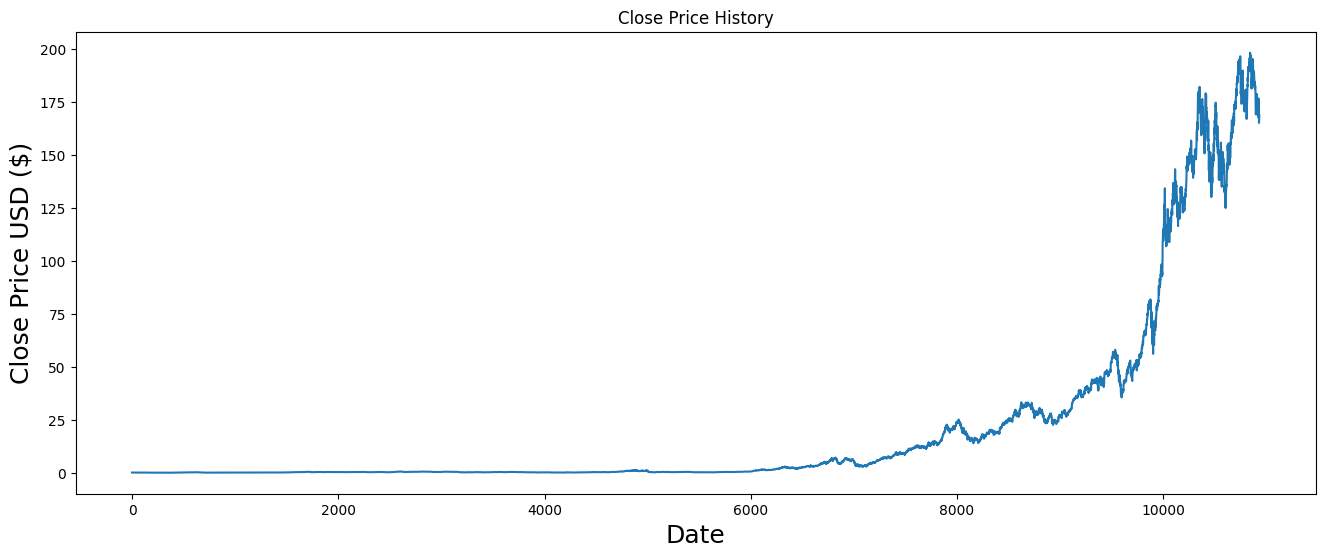
\includegraphics[width=0.45\textwidth]{close_price_history.png}
    \caption{Close Price History of AAPL Stock}
    \label{fig:close-price-history}
\end{figure}

\subsection{Data Scaling}
To get the data ready for LSTM training, we scaled the data with Min-Max scaling. 
This rescales data to a fixed range normally between 0 and 1, which helps to 
stabilize and improve model convergence in training. The idea here is that by 
scaling our data all features have equal footing in learning and no one feature 
overwhelms it during training.

\section{Train/Test Split}
\label{sec:train-test-split}
To prepare the data for training and testing the LSTM model, we split the 
dataset into training and testing sets. The training set will be used to train 
the model, while the testing set will be used to evaluate its performance 
on unseen data.

\subsection{Data Partitioning}
We partitioned the scaled data into training and testing sets using a ratio 
of 95:5, where 95\% of the data was allocated for training and 5\% for testing. 
This ensures that the model is trained on a sufficient amount of data while still 
having unseen data for evaluation.

\subsection{Windowing Approach}
We employed a windowing approach to create input-output pairs for training 
the LSTM model. Each input sequence consists of 60 consecutive closing prices, 
and the corresponding output is the closing price of the next day. This sliding 
window technique allows the model to learn from past observations and 
predict future prices based on historical data.

\subsection{Data Transformation}
After windowing the data, we converted the input-output pairs into numpy 
arrays for compatibility with the LSTM model. The input sequences (\texttt{x\_train} 
and \texttt{x\_test}) were reshaped to have dimensions \texttt{(samples, time steps, features)}, 
where \texttt{samples} represents the number of input sequences, \texttt{time steps} 
represents the number of time steps in each sequence (60 in our case), and \texttt{features} 
represents the number of features (1 in our case, as we only have the closing price).

The following are examples of the input sequences (\texttt{x\_train}) and their corresponding 
output (\texttt{y\_train}):
\begin{itemize}
    \item \textbf{Input Sequence 1}:
    \[
    \begin{bmatrix}
    0.00040008 \\
    0.00036628 \\
    \vdots \\
    0.00025921 \\
    \end{bmatrix}
    \]
    \item \textbf{Output 1}: 0.0002394869529368074
    \item \textbf{Input Sequence 2}:
    \[
    \begin{bmatrix}
    0.00036628 \\
    0.00032119 \\
    \vdots \\
    0.00023949 \\
    \end{bmatrix}
    \]
    \item \textbf{Output 2}: 0.00025920816049633695
\end{itemize}
These input-output pairs were then used to train and test the LSTM model for stock price prediction.

\section{Build LSTM Model}
\label{sec:build-lstm-model}
To construct the LSTM model for stock price  prediction, we utilized the 
Keras library, which provides a high-level interface for building and 
training neural networks. The architecture of the LSTM model consists 
of sequential layers of LSTM and Dense (fully connected) layers.

\subsection{Model Architecture}
The LSTM model was built using the following architecture:
\begin{itemize}
    \item Input Layer: The input layer of the model accepts sequences of closing prices. 
We specified the input shape to be `(timesteps, features)` where `timesteps` corresponds 
to the number of time steps in each input sequence (60 in our case) and `features` 
represents the number of features (1 in our case, as we only have the closing price).
    \item LSTM Layers: We added two LSTM layers with 128 and 64 units, respectively. 
The first LSTM layer returns sequences (return\_sequences=True), while the second 
LSTM layer returns only the output at the last time step (return\_sequences=False).
    \item Dense Layers: We included two Dense layers with 25 and 1 units, respectively. 
The final Dense layer outputs the predicted closing price.
\end{itemize}

\subsection{Model Compilation}
Before training the model, we compiled it using the Adam optimizer and the mean 
squared error (MSE) loss function. Adam optimizer is a popular choice for training 
neural networks due to its adaptive learning rate and momentum. The MSE loss 
function is suitable for regression tasks and measures the average squared difference 
between the predicted and actual values.

\subsection{Model Training}
The compiled model was trained using the training data (\texttt{x\_train} 
and \texttt{y\_train}) for a specified number of epochs and batch size. 
During training, the model learns to minimize the MSE loss by adjusting 
its parameters through backpropagation. The training process involves 
iteratively updating the model's weights to improve its predictive performance.
\texttt{build\_model(batch\_size, epochs)} is a function that we defined in Python
that encapsulates the process of building and training the LSTM model.
This function takes the batch size and number of epochs as input parameters 
and returns the trained LSTM model.



\section{Evaluate Model}
\label{sec:evaluate-model}
To assess the performance of the LSTM model, we evaluated it using 
several metrics commonly used in regression tasks. These metrics provide 
insights into the model's accuracy, precision, and generalization capability.

\subsection{Evaluation Metrics}
We utilized the following evaluation metrics:
\begin{itemize}
    \item \textbf{Mean Squared Error (MSE)}: Measures the average squared difference between the predicted and actual values.
    \item \textbf{Mean Absolute Error (MAE)}: Measures the average absolute difference between the predicted and actual values.
    \item \textbf{Root Mean Squared Error (RMSE)}: Represents the square root of the MSE, providing a more interpretable measure of error.
    \item \textbf{R-squared ($R^2$) Score}: Indicates the proportion of the variance in the dependent variable that is predictable from the independent variable.
\end{itemize}

\subsection{Model Evaluation Function}
 \texttt{evaluate\_model(model, x\_test, y\_test)} is a Python function we defined
to compute these evaluation metrics. The function takes the trained LSTM 
model (\texttt{model}), the testing data (\texttt{x\_test}), and the corresponding 
actual values (\texttt{y\_test}) as inputs. It returns the computed MSE, MAE, RMSE, 
and $R^2$ score.

\section{Optimization}
\label{sec:optimization}
In this section, we explore the optimization of our LSTM model to achieve 
the best performance for predicting stock prices. Optimization involves 
fine-tuning various parameters and configurations to enhance the model's 
predictive capabilities.

\subsection{Epoch Selection}

When training neural networks, such as LSTMS, a critical factor to consider 
is the number of epochs. An epoch is defined as one complete pass through all 
the training examples in the dataset. If we use too few epochs, our model may 
underfit and fail to learn important patterns in the data. On the other hand, 
overfitting can occur when we train for too many epochs; this happens when our 
model memorizes the training set but fails to generalize well on unseen examples.

To determine the optimal number of epochs for our LSTM model, we 
conducted a systematic evaluation across a range of epochs, from 2 to 100, 
with a step size of 2. For each epoch value, we trained the model and evaluated 
its performance using metrics such as MSE, MAE, RMSE, $R^2$.

By analyzing the performance metrics across different epoch values, we identified 
an optimal epoch value, of 25, that strikes a balance between model complexity 
and generalization. This optimal epoch value maximizes predictive accuracy while 
preventing overfitting.

The evaluation results for each epoch value are shown below:

\begin{table}[H]
    \centering
    \begin{tabular}{ccccc}
        \toprule
        \textbf{Epochs} & \textbf{MSE} & \textbf{MAE} & \textbf{RMSE} & \textbf{$R^2$}\\
        \midrule
        2 & 27.255 & 4.312 & 5.221 & 0.916\\
        4 & 22.795 & 3.866 & 4.774 & 0.929\\
        6 & 23.406 & 4.050 & 4.838 & 0.928\\
        ... & ... & ... & ... & ...\\
        26 & 7.919 & 2.137 & 2.814 & 0.975\\
        ... & ... & ... & ... & ...\\
        100 & 8.316 & 2.235 & 2.884 & 0.974\\
        \bottomrule
    \end{tabular}
    \caption{Evaluation Metrics for Different Epochs}
    \label{tab:epoch-metrics}
\end{table}

Finally, we visualize the performance metrics against the number of epochs using a line plot:

\begin{figure}[H]
    \centering
    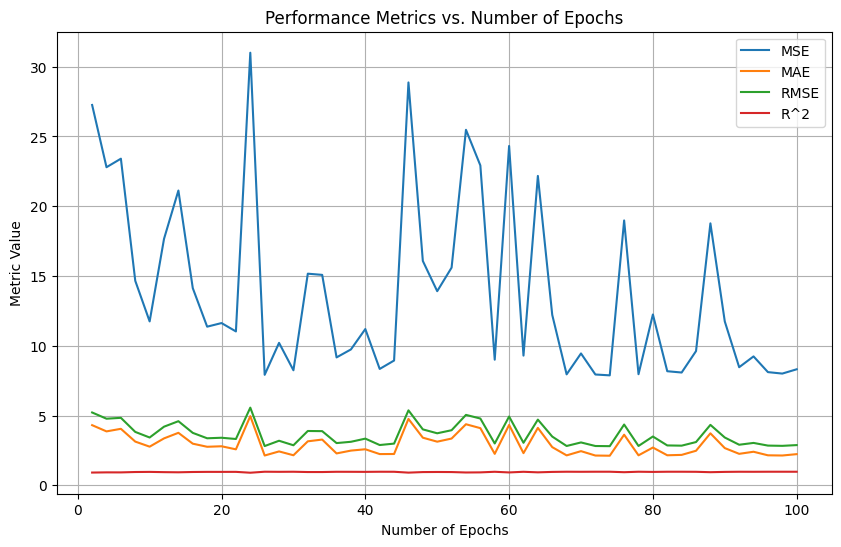
\includegraphics[width=0.45\textwidth]{epoch_metrics_plot.png}
    \caption{Performance Metrics vs. Number of Epochs}
    \label{fig:epoch-metrics-plot}
\end{figure}

From the plot, we can observe the trends of MSE, MAE, RMSE, and $R^2$ score as the 
number of epochs increases. We aim to select the epoch value that achieves the best 
performance based on these metrics.

\subsection{Batch Size Selection}

The batch size is another crucial hyperparameter in training neural networks. It 
represents the number of samples processed before updating the model's parameters 
during training. The choice of batch size can significantly impact the training dynamics, 
convergence speed, and generalization performance of the model.

We systematically evaluated various batch sizes, ranging from 2 to 32, with increments 
of 2. For each batch size, we trained the model and evaluated its performance using 
metrics such as MSE, MAE, RMSE, and $R^2$.

Analyzing the performance metrics across different batch sizes allowed us to identify 
the optimal batch size for our LSTM model. We observed that a batch size of 8 
consistently yielded the best performance across all evaluation metrics. This batch size 
strikes a balance between computational efficiency and model generalization,.

The evaluation results for each batch size value are shown below:

\begin{table}[H]
    \centering
    \begin{tabular}{ccccc}
        \toprule
        \textbf{Batch Size} & \textbf{MSE} & \textbf{MAE} & \textbf{RMSE} & \textbf{R$^2$} \\
        \midrule
        2  & 15.179 & 3.138 & 3.896 & 0.953 \\
        4  & 31.084 & 4.979 & 5.575 & 0.904 \\
        6  & 13.934 & 2.986 & 3.733 & 0.957 \\
        8 & 7.805 & 2.103 & 2.794 & 0.9756 \\
        ... & ... & ... & ... \\
        32 & 9.867  & 2.483 & 3.141 & 0.969 \\
        \bottomrule
    \end{tabular}
    \caption{Performance metrics for selected batch sizes}
    \label{tab:selected_batch_sizes}
\end{table}

Finally, we visualize the performance metrics against the number of batch sizes using a line plot:

\begin{figure}[H]
\centering
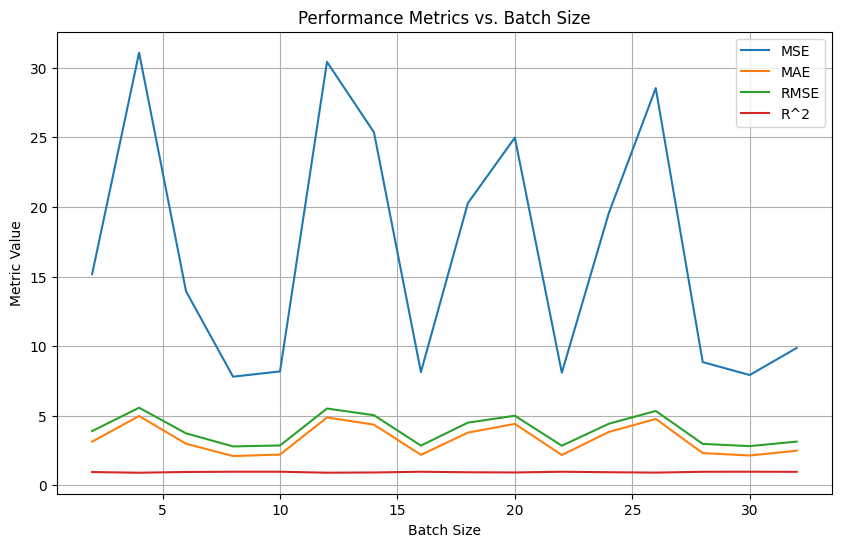
\includegraphics[width=0.45\textwidth]{batch_metrics_plot.png}
\caption{Performance metrics vs. Batch size}
\label{fig:batch_size_performance}
\end{figure}

From the plot, we can observe the trends of MSE, MAE, RMSE, and $R^2$ score as the 
number of batch size increases. We aim to select the batch size value that achieves the 
best performance based on these metrics.

\section{Final Model Evaluation}

After the ideal epoch and batch size are obtained, we build a final LSTM model and train it
for 25 epochs with a batch size of 8.

After training, the model is evaluated, and the following metrics are obtained:

\begin{itemize}
    \item \textbf{MSE}: 8.05
    \item \textbf{MAE}: 2.14
    \item \textbf{RMSE}: 2.84
    \item \textbf{R$^2$}: 0.98
\end{itemize}

The table below shows the actual and predicted closing prices:

\begin{table}[H]
    \centering
    \begin{tabular}{ccc}
        \toprule
        \textbf{Close} & \textbf{Predictions} \\
        \midrule
        164.32 & 167.86 \\
        160.07 & 165.04 \\
        162.74 & 161.02 \\
        164.85 & 163.94 \\
        165.12 & 165.76 \\
        ... & ... \\
        167.04 & 168.56 \\
        165.00 & 167.68 \\
        165.84 & 165.67 \\
        166.90 & 166.63 \\
        168.65 & 167.59 \\
        \bottomrule
    \end{tabular}
    \caption{Actual and predicted closing prices}
    \label{tab:actual_predicted_prices}
\end{table}

Finally, we visualize the predictions of the final model:

\begin{figure}[H]
\centering
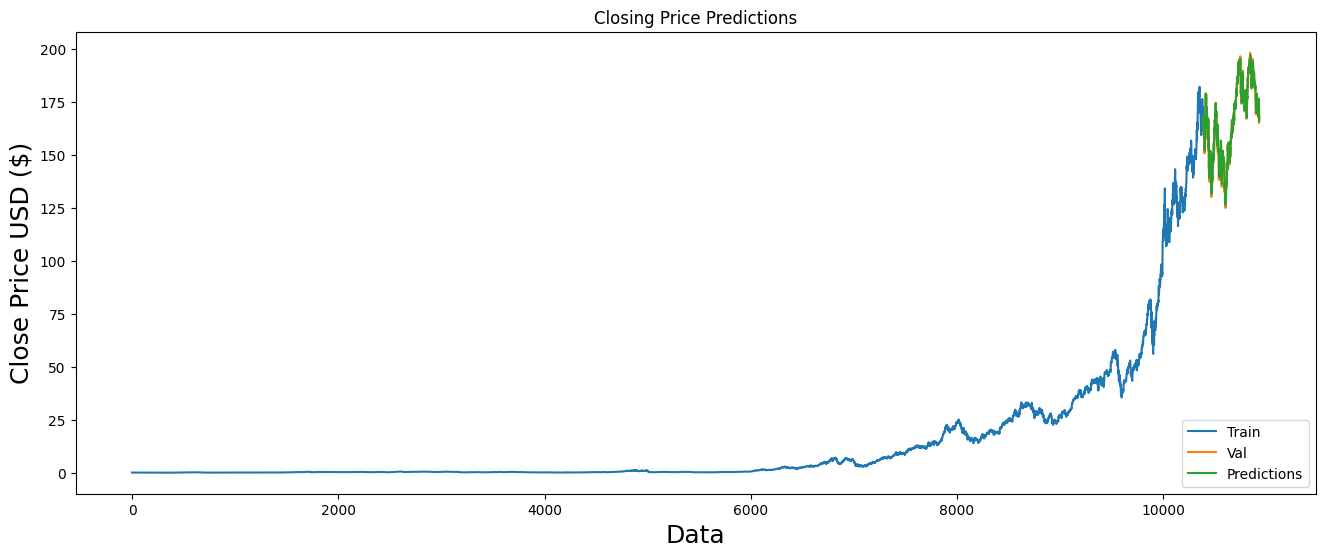
\includegraphics[width=0.45\textwidth]{final_model_predictions.png}
\caption{Predicted Closing Price}
\label{fig:predicted_closing_price}
\end{figure}

After analyzing the performance metrics and examining the actual versus predicted 
closing prices, it's evident that the final LSTM model performs admirably in 
forecasting the stock prices. The mean squared error of 8.05 indicates that, 
on average, the squared differences between the predicted and actual closing prices 
are relatively low. The mean absolute error of 2.14 signifies that, on average, 
the model's predictions deviate from the actual prices by approximately \$2.14. 
Additionally, the root mean squared error of 2.84 provides insight into the 
typical magnitude of the errors in the model's predictions, with lower values indicating 
better performance. Furthermore, an $R^2$ of 0.98 suggests that the model explains 
approximately 98\% of the variance in the dependent variable, which in this case is the 
closing prices. This high $R^2$ value indicates that the model fits the data well and 
captures the underlying patterns effectively.

Examining the table displaying the actual and predicted closing prices further validates 
the model's efficacy. The predictions closely track the actual prices, demonstrating the 
model's ability to capture the trend and fluctuations in the stock prices.

Moreover, the visualization of the predicted closing prices in Figure 
\ref{fig:predicted_closing_price} provides a clear illustration of how well the model predicts 
the trend over time. The plot aligns closely with the actual closing prices, affirming the 
model's accuracy in capturing the underlying patterns in the data.

Overall, based on the performance metrics, comparison of actual versus predicted prices, 
and visualization of the predictions, it can be concluded that the final LSTM model delivers 
robust and reliable forecasts of the stock prices, making it a valuable tool for decision-making 
in financial markets.

\section{Conclusion}

In this study, we developed a Long Short-Term Memory (LSTM) neural 
network model to predict the closing prices of a financial asset based 
on historical data. The model was trained using a sequential architecture 
with two LSTM layers followed by two dense layers. The model was 
trained using the Adam optimizer and mean squared error loss function.

After experimenting with different hyperparameters such as the number 
of epochs and batch size, we found that training the model for 25 epochs 
with a batch size of 8 yielded the best results. The evaluation metrics on 
the test data showed a MSE of 8.05, MAE of 2.14, RMSE of 2.84, and R$^2$
of 0.98.

The visualization of the model's performance on the test data indicated that 
the model's predictions closely followed the actual closing prices. However, 
there were instances where the model's predictions deviated from the actual 
prices, suggesting potential areas for improvement.

Overall, the LSTM neural network model showed promising results in 
predicting the closing prices of the financial asset. Further research could 
focus on fine-tuning the model architecture and exploring additional 
features to enhance its predictive performance.


\section{Project Repository}

The code and resources used in this project are available in the project repository hosted on GitHub. You can access the repository at the following URL:

\url{https://github.com/edisonrhuang/Stock-Prediction-With-LSTM}

{\small
\bibliographystyle{ieee_fullname}
\bibliography{egbib}
}

\end{document}
